\documentclass[a4paper]{article}
\usepackage{geometry}
 \geometry{
 a4paper,
 total={170mm,257mm},
 left=20mm,
 top=20mm,
 }

\usepackage[english]{babel}
\usepackage[utf8]{inputenc}
\usepackage{amsmath}
\usepackage{bm}
\usepackage{graphicx,wrapfig,lipsum}

\usepackage[colorinlistoftodos]{todonotes}
\usepackage{hyperref}






\usepackage{enumitem}
\newcommand{\subscript}[2]{$#1 _ #2$}
\usepackage{listings}
 \usepackage{xcolor}



\hypersetup{
    colorlinks=true,
    linkcolor=blue,
    filecolor=magenta,      
    urlcolor=red,
    pdftitle={An Example},
    pdfpagemode=FullScreen,
    }
\urlstyle{same}


\def\ba{\begin{eqnarray}}
\def\ea{\end{eqnarray}}


\title{ Euclid summer school: Parameter estimation for a polynomial model}

\begin{document}

\maketitle


\section{Analytical solution}

   \begin{figure}[h!]
  \centering
  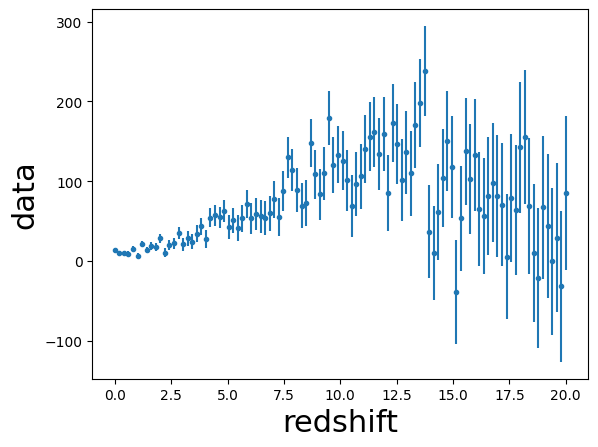
\includegraphics[width=0.5\columnwidth]{data_example.png}
  \caption{The measured data points as a function of redshift}
  \label{fig:data}
\end{figure}


We have access to N measurements of a physical phenomenon that evolves as a function of redshift. Our data model for this phenomenon is an order M polynomial 
\ba
d(z_{i}) = d_{i} =  \sum_{k=0}^{M} a_{k}(z_{i}-z_{c})^{k} + n(z_{i})
\ea
$a_{k}$ are the model parameters that we would like to estimate, $z_i$ are the N redshifts at which the measurements have been done and  $n(z_{i})=n_{i}$ is the noise on the measurements which follows a multivariate gaussian distribution ${\cal N}(0,\Sigma)$. \\
We will assume for now that M=3 and $z_{c}=0$. \\


1) Give an analytic formula for the likelihood of the data given the model parameters ${\cal L}( \{d_{i} \} | \{a_{k} \}) $ (think about the probability distribution  followed by $d_{i} - \sum_{k=0}^{M} a_{k}  (z_{i}-z_{c})^{k}$ \\


2) Download the data file: data\_example.txt, 
 in  \href{https://github.com/thibautlouis/TD/}{here}, the column are redshift, data, error, and reproduce Figure 1. \\


3) For convenience, we will write the data model in vectorial form ${\bm d} = {\cal P}\bm{a} + {\bm n}$   where 
\ba
 {\cal P}= 
 \begin{pmatrix} 
1 &
(z_{0}-z_{c}) & 
(z_{0} -z_{c})^{2}& 
... & 
(z_{0} -z_{c})^{M}
\cr
1 &
(z_{1}-z_{c}) & 
(z_{1} -z_{c})^{2}& 
... & 
(z_{1} -z_{c})^{M}
\cr
... & 
...  &
... & 
... & 
...& 
\cr
1 &
(z_{N-1}-z_{c}) & 
(z_{N-1} -z_{c})^{2}& 
... & 
(z_{N-1} -z_{c})^{M}
\cr
\end{pmatrix}, \
 {\bm a}= 
 \begin{pmatrix} 
a_{0} \cr
a_{1} \cr
... \cr
a_{M} \cr
\end{pmatrix}
\ea



$ {\cal P}$ is a (N $\times$ (M+1)) matrix, write a function that build the matrix ${\cal P}$ using the redshift column of the data file. \\

4) The variance of the noise on the measurement is given by $ \Sigma_{ii} =  \sigma_{0}^{2} + \sigma_{1}^{2} (1+z_{i})^{3}$, with $\sigma_{0} = \sqrt{3}$ and  $\sigma_{1} = 1$   the correlation between the different measurements is null but for adjacent redshifts, in that case it takes the constant value of 0.1

\ba
\rho_{ij} = \Sigma_{ij}/\sqrt{\Sigma_{ii}\Sigma_{jj}}= 0.1& \mbox{only if} & |i-j|=1 
\ea

Write a function that construct the covariance matrix, check that the square root of its diagonal do agree with the error column of the data file, then evaluate the $\chi^{2} = ({\bm d}  - {\cal P}\bm{a})^{T} \Sigma^{-1} ({\bm d}  - {\cal P}\bm{a})$ for the set of parameters $a_{0}= 8$, $a_{1}=3$, $a_{2}=0.4$, $a_{3} = -0.02$,  you should get $\chi^{2} \sim 122.9827$, is this set of parameter a good fit to the data ? \\

5) in our model, the different parameters $a_{k}$ enter linearly in the model,  we can analytically derive the Maximum Likelihood (ML) solution, write down an expression for $\ln({\cal L}({\bm d} |  {\bm a}))$, and show that its extremum is obtained when 
\ba
   \bm{\hat{a}} = ( {\cal P}^{T}  \Sigma^{-1}{\cal P})^{-1}{\cal P}^{T}  \Sigma^{-1} \bm{d} 
\ea
tip: ask for $ \nabla_{ \bm{a} } {\rm ln}{\cal L}(\bm{d} | \bm{a})=0 |_{    \bm{a} =   \bm{\hat{a}}}$
This solution is called the Maximum Likelihood estimate of $\bm{a} $ and is denoted $\bm{\hat{a}}$. \\

6) Show (analytically) that the expectation value of the ML estimator and its covariance are given by

\ba
\langle  \bm{\hat{a}}  \rangle= \bm{a},  \ \ \
{\rm Cov}(\bm{\hat{a}}) &=&  ( {\cal P}^{T}  \Sigma^{-1}{\cal P})^{-1}
\ea

7) Write a function that evaluate the maximum solution corresponding to the provided data file, print the value of the  $\hat{a}_{k}$ parameters and their associated uncertainties. \\

8) Plot the best fit model with respect to the data point, estimate the  $\chi^{2} = ({\bm d}  - {\cal P}\bm{\hat{a}})^{T} \Sigma^{-1} ({\bm d}  - {\cal P}\bm{\hat{a}})$ and p-value of the best fit model. \\

9) Compute the correlation matrix associated with ${\rm Cov}(\bm{\hat{a}}) $ and plot it, you should see that the parameters are pretty correlated.




  % \begin{figure}[h!]
 % \centering
 % 
\includegraphics[width=0.8\columnwidth]{musk.png}
 % \caption{Negociations between Elon musk and Nasa for building a new satellite}
 % \label{fig:data}
%\end{figure}

\section{Monte Carlo verification of the estimator}

A Monte Carlo method designs a numerical method using random processes to estimate numerical quantities. \\

We have written an analytic formula for the maximum likelihood solution to our parameter estimation problem, here we would like to check numerically that the estimator is indeed unbiased and that the analytic covariance formula is indeed correct \\
We will draw simulations of the data,  there is two steps: 1.  Perform a Choleski decomposition of the noise covariance matrix $\Sigma = LL^{T}$, 2. Generate vectors of random gaussian  number, ${\bm u}$, of size N with mean 0 and covariance $\delta_{ij}$. 
A noise simulation will be given by: ${\bm n}^{simu}= L {\bm u} $ \\

1)  Choose a set of parameters $\bm{a}$ and generate a bunch of simulation of the data 

\ba
{\bm d}_{\ \rm sim \ 1} &=& {\cal P} \bm{a} + {\bm n}^{\rm sim 1} \\
&....& \nonumber \\
&....& \nonumber  \\
{\bm d}_{\ \rm sim \  1000} &=& {\cal P}\bm{a} + {\bm n}^{\rm sim 1000}
\ea

for each simulation estimate the maximum solution for  $\bm{a}$, create a list of estimated $\{ \bm{\hat{a}}_{\rm sim 1}, \bm{\hat{a}}_{\rm sim 2}, ...., \bm{\hat{a}}_{\rm sim 1000} \}$ \\

2) Compute the numerical mean and covariances of the list of estimated maximum likelihood parameters, does the mean match your input parameters ? does the numerical covariance matches your analytical formula ? \\

3) For each simulation compute the associated $\chi^{2}$ e.g,  $\chi^{2}_{\rm sim 1 } = ({\bm d}_{\rm sim 1}  - {\cal P}\bm{\hat{a}_{\rm sim 1}})^{T} \Sigma^{-1} ({\bm d}_{\rm sim 1}  - {\cal P}\bm{\hat{a}_{\rm sim 1}})$ and p-value.  \\

4) Display the $\chi^{2}$ distribution of the simulations (plot an histogram with the values of $\{\chi^{2}_{\rm sim 1 }, ..., \chi^{2}_{\rm sim 1000  } \}$ and compare with the expected distribution of $\chi^{2}$ with N-M DoF, do the same with the p-value, what is the expected distribution of p-value ?

% $\nabla_{\bm{a}) \ln({\cal L}(d | \{a_{k} \})$

 \section{Monte Carlo Markov chains}

We have been able to solve this problem analytically, this is due to the fact that the parameters enter linearly in the model, for a more general case we will have to use different methods.
A standard method is Monte Carlo Markov chains, the idea is to design an algorithm that draw samples from the posterior distribution of the parameters. In this section we will code our own MCMC algorithm and redo the parameter estimation of our model. \\

A popular MCMC algorithm is the Metropolis Hasting algorithm, schematically

\begin{enumerate}[label=(\subscript{I}{{\arabic*}})]
\item Define a function $f(\bm{a}) =  {\cal L}({\bm d} |  {\bm a})  P(\bm a)$ \\
\item Choose a starting point for your parameters $\bm a_{0}$ \\
\item Choose a proposal $g({\bm a'}| {\bm a_{0}})$, it is the function that will help us move in the parameter space, a usual choice is a multivariate distribution centered on $\bm a_{0}$ with covariance $ \Sigma=  \frac{2.4^{2}}{D} \rm Cov({\bm{a})}$
\ba
g({\bm a'}| {\bm a_{0}}) = \frac{1}{(2\pi)^{D/2} \sqrt{|\Sigma |}} {\rm exp}  - \frac{1}{2} \left[   
({\bm a'} - {\bm a_{0}})
 \right]^{T} \Sigma^{-1}  \left[   
({\bm a'} - {\bm a_{0}})
 \right]
\ea
\item Randomly draw a candidate ${\bm a'}$ from the proposal
\item Compute the acceptance rate $\alpha = \frac{f(\bm{a'})}{f(\bm{a_{0}})}$ 
\item Draw a uniform random number between 0 and 1 
\ba
u \leq \alpha & \mbox{accept the candidate} & \bm{a_{1}} = {\bm a'}  \\
u > \alpha  & \mbox{reject the candidate} & \bm{a_{1}} = \bm{a_{0}}
\ea
\item Iterate \\

The idea of the algorithm is the following, we explore the parameter space, if we move toward a  state with higher probability, the move is always accepted.
If we move towards a less probable state, the move can be either accepted or rejected, the rejection depends on the ratio of probability between the two points in parameter space. The random walk preferentially explores the parameter space where the posterior is high but occasionally moves in region with lower probability, this helps avoiding being trapped in local maxima.  \\
 



1) Write down a version of the Metropolis Hasting algorithm, and draw $10^{4}$ samples of $\bm{a}$ . \\

2) Plot the corresponding chains. At the beginning of the chains we will notice a "burn in" phase, a phase where parameters value varies by a lot, this should be discarded for later analysis. \\

3) Plot an histogram of the chains, this represents the posterior distribution of our estimated parameters, compare this with the analytical estimate.

4) In practice you won't have to use your own MCMC sampler since many of them are already publicly available, a popular one in cosmology is cobaya an example of how to use cobaya is given below:
 
 

\definecolor{codegreen}{rgb}{0,0.6,0}
\definecolor{codegray}{rgb}{0.5,0.5,0.5}
\definecolor{codepurple}{rgb}{0.58,0,0.82}
\definecolor{backcolour}{rgb}{0.95,0.95,0.92}

\lstdefinestyle{mystyle}{
    language=python,
    backgroundcolor=\color{backcolour},   
    commentstyle=\color{codegreen},
    keywordstyle=\color{magenta},
    numberstyle=\tiny\color{codegray},
    stringstyle=\color{codepurple},
    basicstyle=\ttfamily\footnotesize,
    breakatwhitespace=false,         
    breaklines=true,                 
    captionpos=b,                    
    keepspaces=true,                 
    numbers=left,                    
    numbersep=5pt,                  
    showspaces=false,                
    showstringspaces=false,
    showtabs=false,                  
    tabsize=1
}

\lstset{style=mystyle}



 \begin{lstlisting}
 def cobaya_mcmc(z, data, inv_data_cov, z_c, min_list, max_list, 
 			      chain_name, Rminus1_stop=0.003, Rminus1_cl_stop=0.05):

    from cobaya.run import run

    def log_prob(a0, a1, a2, a3):
        params = [a0, a1, a2, a3]
        model = fp1.generate_model(z, params, z_c)
        res = data - model
        return -0.5 * res @ inv_data_cov @ res

    info = {
        "likelihood": {"my_like": log_prob},
        "params": {
            "a0": {"prior": {"min": min_list[0], "max": max_list[0]}, "latex": "a_{0}"},
            "a1": {"prior": {"min": min_list[1], "max": max_list[1]}, "latex": "a_{1}"},
            "a2": {"prior": {"min": min_list[2], "max": max_list[2]}, "latex": "a_{2}"},
            "a3": {"prior": {"min": min_list[3], "max": max_list[3]}, "latex": "a_{3}"},
        },
        "sampler": {
            "mcmc": {
                "max_tries": 10 ** 8,
                "Rminus1_stop": Rminus1_stop,
                "Rminus1_cl_stop": Rminus1_cl_stop,
            }
        },
        "output": f"{chain_name}",
        "force": True,
        "debug": False,
    }
    

    updated_info, sampler = run(info)
\end{lstlisting}

you can then plot the result using getDist 
 
  \begin{lstlisting}

 def plot_cobaya_chain(chain_name, params):
    from getdist.mcsamples import loadMCSamples
    import getdist.plots as gdplt

    samples = loadMCSamples( f"{chain_name}", settings = {"ignore_rows": 0.5})
    gdplot = gdplt.get_subplot_plotter()
    gdplot.triangle_plot(samples, params, filled = True, title_limit=1)
    plt.savefig(f"{chain_name}.png", dpi = 300)
    plt.clf()
    plt.close()
\end{lstlisting}
\end{enumerate}







\end{document}